\section{Conception \& Architecture}
\subsection{Technologies utilisées}
\subsubsection{Java 8}
Parmi les deux langages de haut niveau proposés pour l'élaboration de ce projet (Java ou C++), nous avons choisi Java pour sa portabilité, sa sécurité et ses performances. De plus, la dernière version de Java propose la librairie graphique JavaFX qui convient parfaitement à notre projet. Enfin, notre équipe est également plus habile à programmer à l'aide du langage Java.

\subsubsection{JavaFX 8}
JavaFX, successeur de Swing, est la librairie de création d'interface graphiques officielle de Java. La version 8, utilisée pour ce projet, ajoute de nouvelles fonctionnalités et est la plus récente version utilisable avec Scene Builder.

JavaFX propose énormément de fonctionnalités, passant par la création d'interface à la modélisation d'objet 3D. Dans notre projet, nous allons utiliser les composants de base permettant de créer des interfaces simples. Nous utiliserons également le langage CSS afin de mettre en forme l'interface, comme le permet JavaFX.

\subsubsection{Scene Builder 8.3.0}
Scene Builder de Gluon permet de manipuler des objets JavaFX graphiquement et exporter ceux-ci dans un fichier \texttt{.fxml} interprétable par la librairie graphique. L'interface de base a été conçue lors de l'élaboration du cahier des charges pour présenter un exemple de l'interface de l'application finale. Plusieurs maquettes ont été présentées et c'est sur la base de ces dernières que nous avons construit, grâce à Scene Builder, une base d'interface sur la laquelle nous avons rajouté des composants et fonctionnalités tout au long de l'élaboration de l'application. La flexibilité de JavaFX permet d'ajouter des éléments via un fichier externe \texttt{.fxml} mais aussi directement dans le code, ce que nous avons aussi utilisé.

\subsubsection{Maven}
Pour la compilation du projet et l'importation aisée de celui-ci dans un nouvel environnement de travail, nous avons utilisé l'outil Maven de Apache. Il permet de spécifier les dépendances d'un programme ainsi que des instructions permettant de compiler les fichiers source en fichiers exécutables. Ces instructions se trouvent dans le fichier \texttt{pom.xml} et est librement modifiable par les développeurs.


\subsubsection{Git}
Git est un logiciel de gestion de version utilisé pour permettre de stocker tous les fichiers du projet ainsi que toutes les modifications leur ayant été apportées depuis leur création. Pour chaque nouvelle fonctionnalité, nous avons procédé par la création d'une branche à partir de la branche principale (une version fonctionnelle du programme, contenant les fonctionnalités implémentées et testées). Ces nouvelles branches permettent de développer les fonctionnalités du programme indépendamment et de les ajouter à la branche principale une fois inspectées et testées par plusieurs membres de l'équipe.

\subsubsection{GitHub}
Github est un service web permettant de parcourir visuellement l'historique Git et qui fournit également des outils de gestion de Git. Notamment, pour chaque fonctionnalité ou chaque bug découvert, une \og{} issue \fg{} (un problème) peut être ouverte et assignée à un ou plusieurs membres de l'équipe. Dès la fin de l'élaboration du planning de notre projet, des issues ont été assignées à chaque développeur. Celles-ci ont permis de mieux se fier au planning et toujours avoir en vue ce qu'il restait à implémenter.

\subsection{Comparaison de l'interface finale avec la maquette}
La maquette de l'interface à été conçue au début du projet en tenant compte de toutes les fonctionnalités que le programme devait fournir. Les figures \ref{fig:cat_mockup} et \ref{fig:cat_gemms} ci-dessous proposent une comparaison entre la maquette et le résultat final.

\begin{figure}[!ht]
	\caption{Maquette de l'interface}
	\centering
	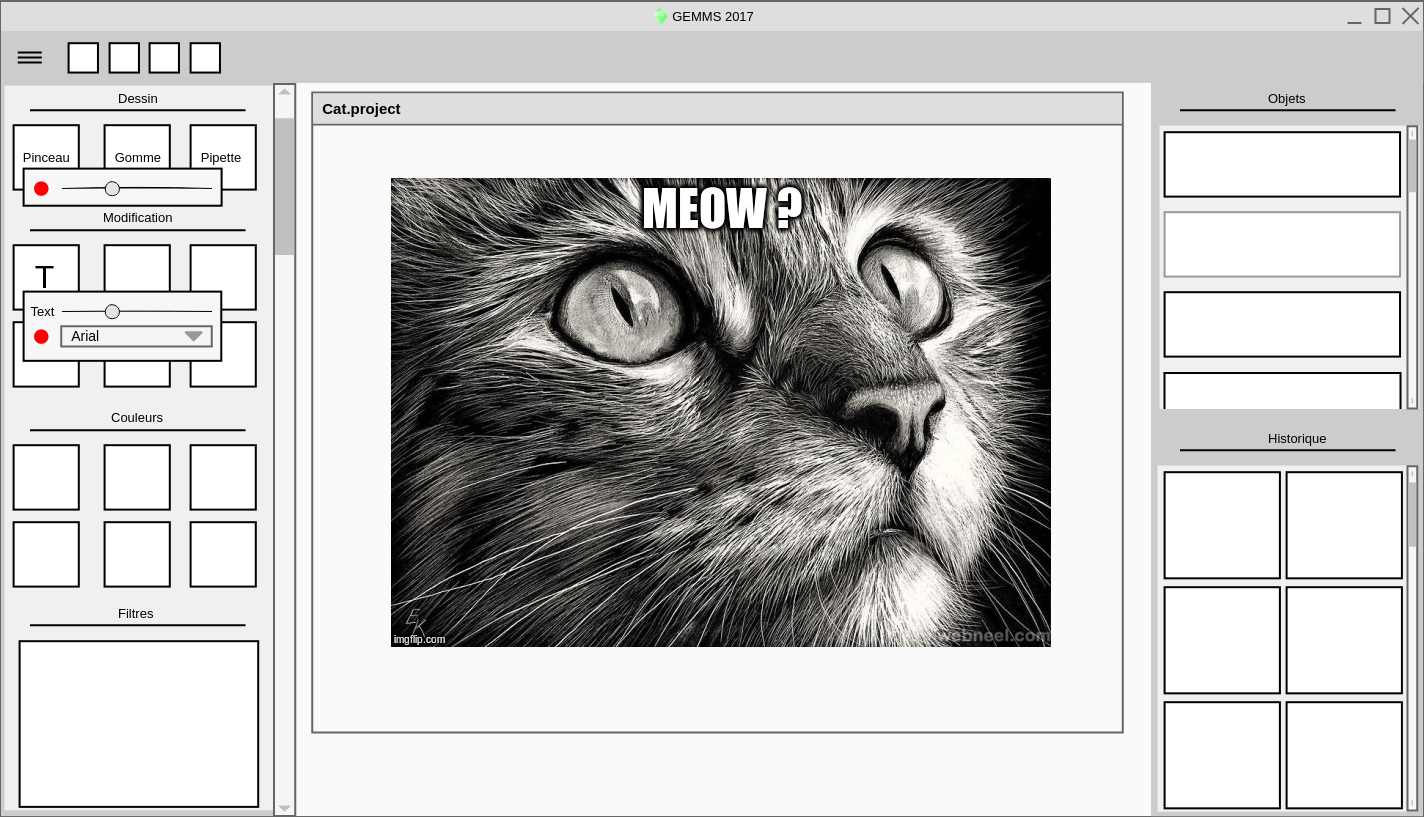
\includegraphics[scale=0.35]{Cat_MOCKUP.png}
	\label{fig:cat_mockup}
\end{figure}

\begin{figure}[!ht]
	\caption{Interface finale du programme}
	\centering	
	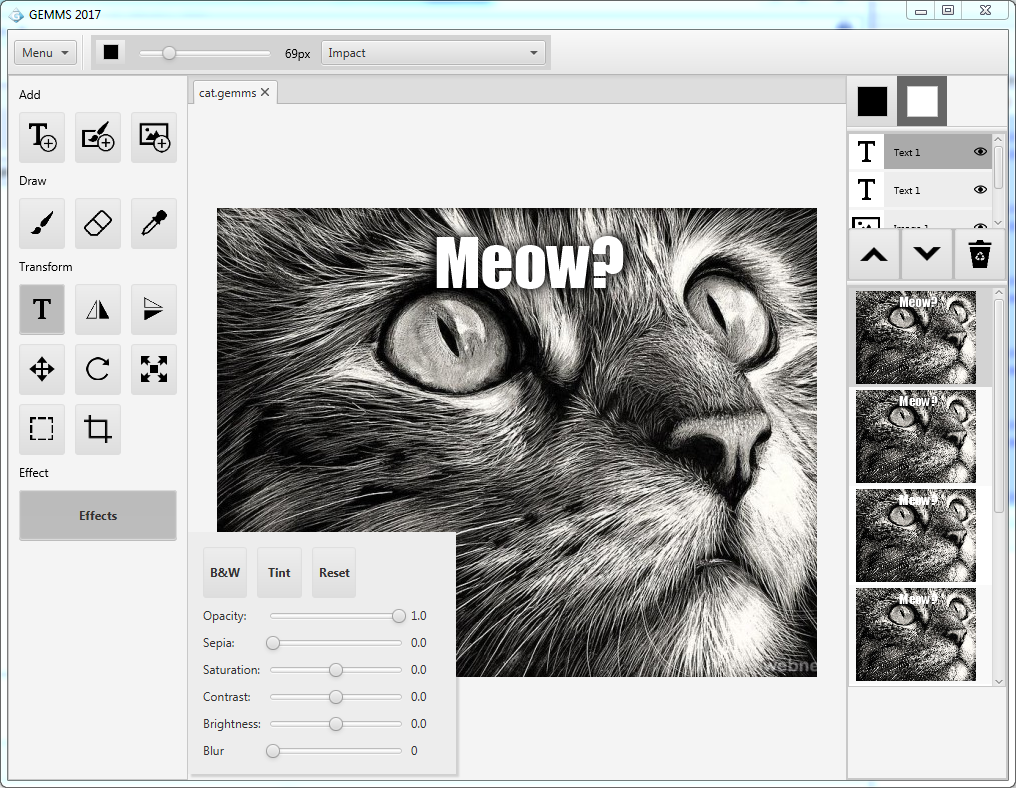
\includegraphics[scale=0.6]{Cat_GEMMS.PNG}
	\label{fig:cat_gemms}
\end{figure}

Comme le montrent les figures \ref{fig:cat_mockup} et \ref{fig:cat_gemms}, l'interface conçue lors de l'élaboration du cahier des charges à été repris presque entièrement pour notre programme. Les différences majeurs sont les paramétrages des outils, qui ont lieu en haut de l'interface à coté du menu déroulant, ainsi que les filtres \& effets, qui ont lieu dans une fenêtre qui peut être ouverte ou fermée à souhait pour rendre l'interface moins chargée. 
\newpage